\documentclass[a4paper,11pt,titlepage]{article}
\usepackage[utf8]{inputenc}
\usepackage{lmodern} \usepackage[T1]{fontenc}
\usepackage[babel=true]{microtype}
\usepackage[portuguese]{babel}
\usepackage[pdftex]{hyperref}
\usepackage{graphicx}
\usepackage{eurosym}
\usepackage{scrextend}
\usepackage{hyphenat}
\usepackage{url}
\usepackage{hyperref}
\usepackage{listings}
\usepackage{indentfirst}
\usepackage{float}
\usepackage[usenames,dvipsnames,svgnames,table]{xcolor}

\lstdefinestyle{customc}{
  belowcaptionskip=1\baselineskip,
  breaklines=true,
  xleftmargin=\parindent,
  language=C,
  showstringspaces=false,
  tabsize=2,
  basicstyle=\footnotesize\ttfamily,
  keywordstyle=\bfseries\color{blue},
  commentstyle=\itshape\color{gray},
  identifierstyle=\color{black},
  stringstyle=\color{OliveGreen},
}

\lstdefinestyle{customcwithlines}{
  belowcaptionskip=1\baselineskip,
  breaklines=true,
  xleftmargin=\parindent,
  language=C,
  showstringspaces=false,
  numbers=left,
  tabsize=2,
  basicstyle=\footnotesize\ttfamily,
  keywordstyle=\bfseries\color{blue},
  commentstyle=\itshape\color{gray},
  identifierstyle=\color{black},
  stringstyle=\color{OliveGreen},
}

\title{\huge \textbf{Aplicação de download e configuração e estudo uma rede\\[1cm] \Large Relatório\\[0.7cm]

\includegraphics{res/logo.png}\\[0.7cm] \large Redes de Computadores\\[0.25cm] \small $3^o$ ano\\[0.05cm]Mestrado Integrado em Engenharia Informática e
Computação\\[1cm]}\normalsize Turma 4}

\author{Carolina Moreira\\Daniel Fazeres\\José Peixoto \and 201303494\\201502846\\200603103 \and  up201303494@fe.up.pt\\up201502846@fe.up.pt\\ei12134@fe.up.pt}

\begin{document}
\maketitle

\newpage
\tableofcontents
\newpage

\abstract
\iffalse dois parágrafos: um sobre o contexto do trabalho; outro sobre as
principais conclusões do relatório \fi

No âmbito da unidade curricular de Redes de Computadores, foi-nos proposto o
desenvolvimento de uma aplicação que permitisse o download de ficheiros usando a especificação de FTP e a configuração e estudo de uma rede de computadores.

\section{Aplicação de download}
A primeira parte do segundo trabalho laboratorial consistiu no desenvolvimento
de uma aplicação de download recorrendo ao protocolo de transferência de
ficheiros FTP especificado pelo \texttt{RFC959}. Para este efeito foi também
necessário resolver o endereço de IP para um dado URL de acordo com
especificação RFC1738. Separaram-se as componentes do parsing do URL e do
cliente de download usando o protocolo FTP respectivamente nos ficheiros
\texttt{url.c} e \texttt{ftp.c}.

\subsection*{Casos de uso principais}
\iffalse (identificação; sequências de chamada de funções) \fi
O programa implementa uma versão básica de um cliente de FTP com suporte para
download de ficheiros de forma anónima ou para um dado par utilizador e
password, introduzidos antecipadamente ao caminho de URL do ficheiro.  Apesar
da introdução do nome de utilizador seguido de password serem facultativos, em
alguns casos tornam-se obrigatórios na transferência com sucesso de um ficheiro
por FTP caso este não esteja disponível de forma pública e requeira
autenticação por parte do utilizador.

\begin{figure}[H]
    \center
    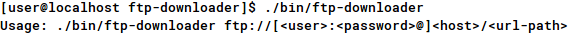
\includegraphics[scale=0.6]{res/usage.png}
    \caption{Utilização do programa}
    \label{fig:usage.png}
\end{figure}

\subsection*{Análise de URL}
Após a leitura e compreensão do \texttt{RFC1738}, desenhou-se uma estrutura de
dados com a finalidade de armazenar a informação extraída da análise de um link
URL recebido pela linha de comandos. Quando fornecidos, são guardados na
estrutura referida, o nome de utilizador, a password, o host, ip, path e nome
do ficheiro em arrays de caracteres independentes. Para além disso, é também
definida a porta 21 como a predefinida na ligação de controlo do protocolo de
FTP. À semelhança do que é referido no \texttt{RFC1738}, caracteres
capitalizados são interpretados como caracteres minúsculos, admitindo ftp da
mesma forma que FTP.

Para se poder resolver o endereço de IP armazenado na estrutura de URL, é feita
uma chamada à função \texttt{gethostbyname} que permite a obtenção do endereço
de uma máquina a partir do nome e retorna uma estrutura do tipo
\texttt{hostent} contendo o endereço na variável \texttt{h\_addr} que é
posteriormente convertido para um array de chars com o auxílio da função
\texttt{inet\_ntoa}.

\subsection*{Cliente de FTP}
O cliente de FTP liga-se através de um socket TCP ao servidor de FTP
identificado pelo endereço de IP acima mencionado e à porta 21 e estabelece uma
ligação de controlo de comunicação, comunicando com uma sequência de comandos
de transferência FTP que lhe são enviados ao estilo do protocolo Telnet: 

\begin{labeling}{alligator}
\item [\textbf{USER user}] envio do nome de utilizador sob a forma de uma string que identifica o utilizador no servidor remoto.
\item [\textbf{PASS pass}] envio da palavra passe completando a identificação no sistema de identificação e controlo de acesso do servidor.
\item [\textbf{CWD path}] indicação do directório que contém o ficheiro requerido para download e sobre o qual se pretende trabalhar.
\item [\textbf{PASV}] comando que pede ao servidor para ficar à escuta numa porta de dados diferente da porta usada pelo serviço de controlo. Este comando recebe uma resposta que contém o endereço e a porta na qual o servidor ficou à escuta para poder estabelecer uma outra ligação TCP usada para transferência de dados.
\item [\textbf{RETR filename}] comando \texttt{retrieve} que pede ao servidor que inicie a transmissão de uma cópia do ficheiro especificado pelo campo \texttt{filename} usando a nova ligação estabelecida ao endereço e porta recebidos pelo comando anterior.
\end{labeling}

Uma vez estabelecida a ligação dedicada de transmissão de dados, estes vão
sendo recebidos de forma ordenada pelo cliente de FTP e armazenados em disco.

\subsection*{Casos de uso}
Um possível caso de uso pode ser o download de um ficheiro de forma anónima do
URL \texttt{ftp://ftp.up.pt/pub/CentOS/filelist.gz}:

\begin{figure}[H]
    \center
    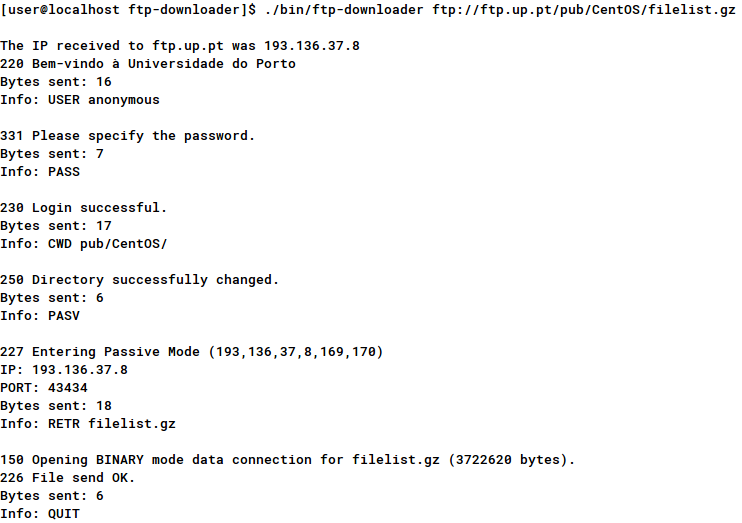
\includegraphics[scale=0.45]{res/anonymous.png}
    \caption{Utilização anónima para download de um ficheiro}
    \label{fig:anonymous.png}
\end{figure}

Também foi testado o download de um ficheiro quando é requerida a autenticação
do utilizador no servidor de FTP:

\begin{figure}[H]
    \center
    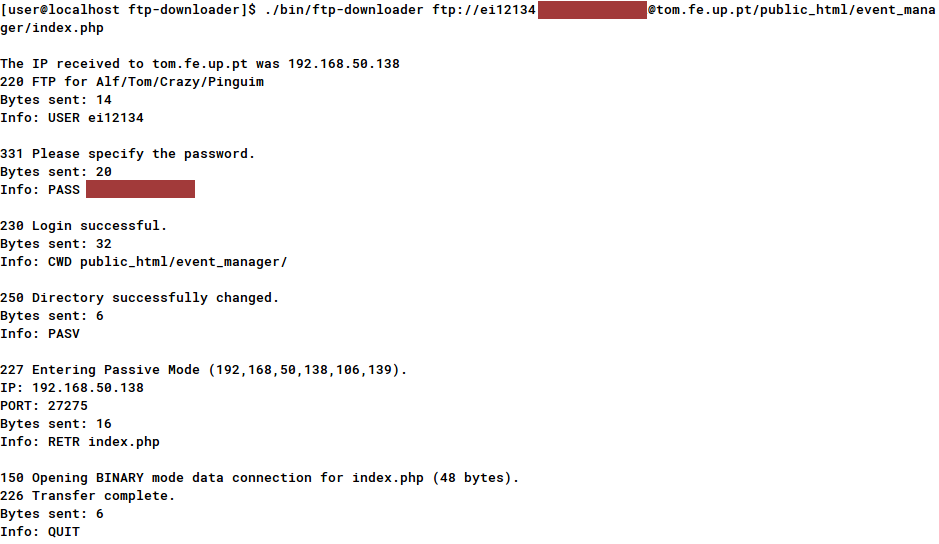
\includegraphics[scale=0.45]{res/authenticated.png}
    \caption{Utilização autenticada no download de um ficheiro}
    \label{fig:authenticated.png}
\end{figure}

\section{Experiência 1: Configuração de uma rede IP }

Nesta experiência, configuraremos apenas uma rede simples de dois computadores
ligados entre si por um switch. Esta rede usará o conjunto de protocolos que
constituem, em parte, a arquitectura da mais conhecida rede de todas, a
Internet. Como é sabido, o protocolo que gere a camada de rede da Internet é
o IP (Internet Protocol).  Para além do próprio protocolo IP, a Internet usa
vários outros protocolos auxiliares para regular o seu funcionamento,
nomeadamente ARP, ICMP, e DHCP.
O protocolo DHCP é usado para negociar automaticamente a atribuição de um
endereço IP a qualquer elemento de uma rede que permita uma identificação única
perante outros membros. Este protocolo não será usado, e em vez disso
atribuir-se-á manualmente e estaticamente endereços IP a cada um dos
computadores das redes desta e subsequente experiências deste trabalho, o que é
exequível visto tratarem-se de redes de pequena dimensão, o que não seria o
caso noutras instalações de aplicação prática no mundo real.

Os endereços desta experiência serão divididos, como é feito neste protocolo de
rede, numa parte respeitante à subrede (subnet), e outra que indicará o
endereço de cada computador dentro desta rede. Um pequeno esquema do resultado
pretendido é indicado na próxima imagem.

\begin{figure}[H]
    \center
    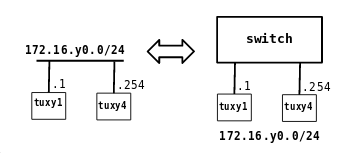
\includegraphics[scale=0.45]{res/network1.png}
    \caption{Rede da 1a Experiência}
    \label{fig:network1.png}
\end{figure}

\subsection*{Configuração de interfaces}

Na configuração desta rede, começamos por ligar apenas os computadores TUX1 e
TUX4 ao switch Cisco Catalyst 3560. Cada um dos computadores tem duas
interfaces expostas, para além da loopback.
A interface loopback é uma interface apresentada pelo sistema operativo como
qualquer outra interface, mas possuíndo o endereço especial $127.0.0.1$
(IPv4) e $::1$ (IPv6). Pacotes dirigidos a este endereço são direccionados para o
próprio computador.
Cada interface pode ser configurada independentemente das outras, e o software
de rede do sistema operativo encarregar-se-á de encaminhar o tráfego de rede
para uma ou outra consoante a rede a que pertence e o destino do tráfego. Por esta razão, e uma vez que a configuração será manual, atribuiremos um endereço IP
juntamente com uma máscara de rede à interface eth0 destes TUXs.

O primeiro passo é desactivar a interface eth1 com o comando

$$ifconfig\ eth1\ down$$

Numa nota à parte, este relatório foi completado depois de uma
reconfiguração dos computadores por parte dos responsáveis pela manutenção do
laboratório, pelo que, no caso de alguns TUXs, o programa usado para configurar
as interfaces foi o $ip$ e não o $ifconfig$, para o qual os comandos são
diferentes. Para desactivar esta interface com o $ip$ usámos o comando

$$ip\ link\ set\ eth1\ down$$

Seguidamente, removemos os IPs atribuídos ao TUX1 com:

$$ip\ addr\ flush\ dev\ eth0$$

após o que atribuímos o endereço pretendido:

$$ip\ addr\ add\ 172.16.10.1/24\ dev\ eth0$$

e confirmamos o resultado com:

$$ip\ addr\ show\ [dev\ eth0]$$

% inserir aqui resultados do comando
Nos resultados podemos ver a interface loopback já mencionada, o IP que
configurámos na interface eth0, e que a MTU desta interface é 1500 bytes, que é
o tamanho máximo de uma frame em ethernet, que é o tipo de rede (camada de
rede) que estamos a utilizar.
Realizamos o mesmo procedimento no TUX4, atribuindo o endereço IP com:

$$ifconfig\ eth0\ 172.16.10.254/24$$

\subsection*{Configuração do switch}

O próximo passo é configurar o switch que liga os dois computadores.  Para
aceder à sua configuração, ligamos o seu terminal a um adaptador cuja saída é
uma ligação em série, que depois é ligada à entrada de porta de série do TUX1,
exposta no ficheiro $/dev/ttyS0$ do mesmo.
Para termos a certeza que não existem configurações já definidas a interferir no nosso trabalho, fazemos reset do switch. Utilizando o programa $gtkterm$ para
comunicar com a sua linha de comandos, começamos por entrar em modo de
configuração com o comando $enable$, para o qual precisamos de introduzir a
password do switch. Escrevemos, depois, os comandos:

$$copy\ tftp://192.168.109.1/2\ startup-config$$
$$delete\ flash:vlan.dat$$
$$reload$$

\subsection*{Rotas}

O comando $reload$ demora algum tempo a terminar. Durante este intervalo,
podemos verificar as rotas de cada um dos computadores com o programa
$route$.
Podemos observar que temos uma única entrada para interface na sua tabela.)
A coluna de destino (Destination) juntamente com a máscara de rede (Genmask),
determinam para que endereços a sua linha será aplicada. Neste caso, visto a
máscara de rede ser $255.255.255.0$ (ou seja, usamos os primeiros três grupos
de 8 bytes, ou 24 bits, conforme indicámos nos comandos anteriores), esta
entrada será usada para todos os IPs que começam por $172.16.10$.
Um valor de Gateway nesta tabela indica que o pc enviará pacotes para o endereço de destino directamente em vez de um intermediário, que é o predendido, visto
estarem ambos ligados entre si. O switch utilizado redireciona pacotes para as
entradas apropriadas, verificando os IPs (é um switch activo ao invés de
passivo), mas não recebe pacotes como se fosse um host normal -- ou seja, a sua
existência é transparente no processo de routing -- por isso não aparece nesta
tabela de routing.

\subsection*{VLAN}

No entanto, para ter os TUXs a comunicar entre si, temos de nos assegurar que
estão na mesma VLAN (a VLAN 1, default) do switch. Podemos inspeccionar isto
com o comando $show\ vlan\ brief$ no switch em modo normal.

% escrever aqui resultados do switch

Ligámos o TUX1 à entrada 1 do switch, que a designa por $Fa0/1$ (abreviatura de
Fastethernet 1, visto ser uma entrada de Fastethernet) e o TUX2 à entrada dois.
Nos resultados do switch, vemos que estão os dois na mesma rede.

\subsection{Pacotes ARP e endereços MAC}

Em qualquer rede deste tipo, o protocolo \emph{ARP} (Address Resolution Protocol)
desempenhará a função necessária de comunicar a atribuição de endereços IP
entre vizinhos -- NICs (Network Interface Cards), como placas Ethernet, não
compreendem endereços IP, emitindo apenas tramas endereçadas pelo ao que se
chamam endereços MAC (Media Access Control), atribuídos pela IEEE e
garantidamente únicos em qualquer parte do mundo. Quando um computador numa
rede deste tipo deseja saber a que endereço MAC corresponde um determinado
endereço IP, emite (através de broadcast) um pacote ARP com a pergunta "a quem
pertence este endereço IP?". De seguida, o dono do endereço referido responde à
questão com outro pacote. O emissor do primeiro pedido de ARP também inclui o
seu próprio endereço IP na mensagem, eliminando a necessidade do segundo membro
da rede perguntar ele próprio para que endereço de IP deve responder.
De notar que os pacotes utilizados nesta troca são pacotes IP, e não
simplesmente tramas de Ethernet.

Cada membro da rede mantém em cache uma tabela de atribuições de endereços IP,
mas esta deve ter uma duração finita, para lidar com reconfigurações na rede e
na sua topologia. Quando um computador é configurado inicialmente, pode emitir
um pedido ARP pelo seu próprio endereço. Não deverá ocorrer nenhuma resposta,
mas todos os seus vizinhos deverão receber a informação relativa ao endereço IP
do emissor.

Este protocolo é definido no RFC 826.

Para podermos observar pacotes ARP, apagaremos a tabela de ARP dos dois
computadores com o comando $arp\ -d$.

\subsection{Comandos PING}

% escrever aqui teoria sobre IMCP

\section{Experiência 2: Duas VLANs num switch}

Nesta experiência foram configuradas duas VLAN's no switch. A primeira VLAN é constituída pelo TUX1 e pelo TUX4 e a segunda pelo TUX2. Criou-se no switch a vlan0 e adicionou-se as portas correspondentes ao TUX1 e TUX4. Criou-se a vlan1 e adicionou-se a porta correspondente ao TUX2. Para adicionar uma nova VLAN ao switch acedeu-se pela consola de configuração e executou-se o comando \texttt{vlan [n]}. Após a criação da VLAN foi-se adicionando as portas do switch associadas com o comando \texttt{interface fastethernet 0/[i]}, seguido do comando \texttt{switchport access VLAN [n]}.

Uma vez configuradas as VLANs, testou-se a nova configuração pingando o TUX2 quer da TUX1 quer do TUX4. Como o TUX2 faz parte de uma sub-rede diferente, o comando falhou como seria de esperar.

\section{Experiência 3: Configurar um router em Linux}
Nesta experiência configurou-se o TUX4 por forma a transformá-lo num router que faz de ponte entre as duas sub-redes atrás mencionadas. Configurou-se a segunda carta de rede \texttt{eth1} do TUX4 atribuindo-lhe o IP 172.16.11.253 pertencente à segunda sub-rede.
Adicionaram-se as rotas apropriadas ao TUX1 e ao TUX2 para que conseguissem comunicar entre si. Para o efeito, no TUX1 executou-se o comando \texttt{route add -net 172.16.11.0/24 gw 172.16.10.254} em que o primeiro endereço identifica a gama de endereços para a qual se quer adicionar a rota e o segundo, é o endereço IP do TUX4 para o qual se deve reencaminhar o pacote. AO TUX2 adicionou-se a nova rota com o comando \texttt{route add -net 172.16.10.0/24 gw 172.16.11.253}, em que o IP 172.16.11.253 é o IP previamente atribuído ao TUX4 nesta segunda sub-rede. Por fim, pingou-se com sucesso o TUX2 a partir do TUX1 e vice-versa, confirmando a configuração como correcta, na qual os pacotes são reencaminhados da entre as sub-redes com o recurso ao TUX4 que opera como um router.

\section{Experiência 4: Configurar um router comercial e implementar NAT}
Nesta experiência pretendia-se configurar um router comercial e implementar NAT. Para o efeito, ligou-se o router a uma porta do switch e adicionou-se esta porta à configuração da segunda VLAN atrás referida. Acedeu-se ao router usando a consola de configuração e executou-se o comando \texttt{interface fastethernet 0/0} para configurar esta interface e atribuiu-se o IP para o router na VLAN1 de 172.16.11.254 com o comando \texttt{ip address 172.16.11.219 255.255.255.0}. De seguida, configurou-se a interface externa atribuindo-lhe o IP com o comando \texttt{ip address 172.16.1.19 255.255.255.0}. Para assegurar a atribuição de uma determinada gama de endereços executaram-se os comandos: \texttt{ip nat pool ovrld 172.16.1.19 172.16.1.19 prefix 24} e \texttt{ip nat inside source list 1 pool vorld overload}. Definiram-se também rotas internas e externas com o comando \texttt{ip route 0.0.0.0 0.0.0.0 172.16.1.254} e \texttt{ip route 172.16.10.0 255.255.255.0 172.16.11.253}. Este comando redireciona os pacotes que tenho IP de destino dentro da gama 172.16.10.0-255 para o IP 172.16.11.253.

\section{Experiência 5: DNS}
Nesta experiência pretendia-se configurar o domain name system conhecido pela abreviatura \texttt{DNS}. Este serviço permite que um endereço de domínio seja traduzido num endereço IP válido correspondente. Por exexemplo \texttt{www.google.pt} pode ser traduzido para o endereço de IP \texttt{195.8.12.84}.

\subsection{Como configurar um serviço DNS?}
Para configurar o serviço de DNS adicionou-se uma linha contendo o endereço de um servidor de DNS ao ficheiro de configuração das rotinas de resolução de endereços da internet da biblioteca de C localizado em \texttt{/etc/resolv.conf}.

$$nameserver\ 172.16.1.1$$

A palavra-chave \texttt{nameserver} é seguida do valor que neste caso é um endereço de IPv4 para um servidor de DNS.

\subsection{Pacotes usados por DNS}
Para testar a configuração atrás referida, usou-se o comando ping para o endereço de domínio \texttt{www.google.pt} e observou-se quer o output na linha de comandos quer os pacotes trocados com o servidor de DNS usando o wireshark.
É feito um pedido ao servidor de DNS para que este lhe forneça informações que tenha acerca do endereço de domínio enviado, neste caso \texttt{www.google.pt} e o servidor responde com o tempo de vida, o tamanho dos dados e com o valor do endereço de IP neste caso com 4 byes e com o valor do endereço de IP.

\begin{labeling}{alligator}
\item DNS query:
$$www.google.pt:\ type\ A,\ class\ IN$$

\item DNS answer:
$$www.google.pt:\ type\ A,\ class\ IN,\ addr\ 195.8.11.212$$

\end{labeling}

\section{Experiência 6: Ligações TCP}
Nesta experiência compilou-se a aplicação apresentada no início do relatório com o fim de efetuar uma transferência de um ficheiro alojado num servidor de ftp e analisar o tráfego de rede usando o Wireshark. Uma vez finalizado o download do ficheiro, verificou-se a sua integridade, confirmando que continha os dados que eram expectáveis, confirmando deste modo que a transferência tinha sido feita sem problemas. Este download com successo também permitiu confirmar que era possível resolver um endereço de domínio e aceder a um IP externo a rede configurada. Analisando o tráfego, detetaram-se pelo menos duas ligações de TCP uma que corresponde à ligação de controlo e outra para transfência de dados FTP-DATA. Averiguou-se também que o TCP utiliza o Selective Repeat ARQ, em que o receptor continua a processar frames recebidos mesmo quando detecta algum erro.

\section{Conclusões}
\iffalse (síntese da informação apresentada nas secções anteriores; reflexão
sobre os objectivos de aprendizagem alcançados) \fi

Findo o projeto, consideramos que atingimos os objetivos básicos estipulados. Esta
abordagem prática permitiu uma melhor consciência do funcionamento e configuração de uma rede.

\begin{thebibliography}{9}
\bibitem{lamport93}
  Andrew S. Tanenbaum,
  David J. Wetherall,
  \emph{Computer Networks},
  Prentice Hall, 
  5th edition,
  2011.
\bibitem{rfc1958}
  Network Working Group,
  \emph{Architectural Principles of the Internet},
  June 1996.
\end{thebibliography}

\appendix
\section{Código fonte}
\subsection*{main.c}
\begin{lstlisting}[style=customcwithlines]
#include "ftp.h"
#include "url.h"

#include <stdio.h>
#include <stdlib.h>

#define INVALID_PORT -1
#define USE_IPV6 0

void print_usage(char* program)
{
    fprintf(stdout,
            "Usage: %s ftp://[<user>:<password>@]<host>/<url-path> \
            [-p PORT]\n",
            program);
}

int get_url_from_args(int argc, char** argv, url* dest_url)
{
    int port_option = INVALID_PORT;
    char* url_option = NULL;
    if (argc == 1) {
        print_usage(argv[0]);
        return 1;
    }

    for (int i = 1; i < argc; ++i) {
        if (strcasecmp(argv[i], "-p") == 0) {
            if (argc != 4 || i == argc - 1) {
                print_usage(argv[0]);
                return 1;
            }
            i += 1;
            for (char* s = argv[i]; *s != '\0'; ++s) {
                if (!isdigit(*s)) {
                    print_usage(argv[0]);
                    return 2;
                }
            }
            port_option = atoi(argv[i]);
        } else {
            url_option = argv[i];
        }
    }

    // Uniform resource locator parser
    url url;
    init_url(&url);
    if (parse_url(&url, url_option))
        return -1;

    if (USE_IPV6) {
        if (get_host_ipv6(&url)) {
            printf("Error: Cannot find ip to hostname %s.\n", url.host);
            return -1;
        }
    } else {
        if (get_host_ipv4_new(&url)) {
            printf("Error: Cannot find ip to hostname %s.\n", url.host);
            return -1;
        }
    }

    if (port_option != INVALID_PORT) {
        url.port = port_option;
    }
    *dest_url = url;

    return 0;
}

void abort_connection(ftp* ftp, char* msg, int ret)
{
    //fprintf(stderr,msg);
    printf(msg);
    disconnect_ftp(ftp);
    exit(ret);
}

int main(int argc, char** argv)
{
    url url;
    int get_url_ret = get_url_from_args(argc, argv, &url);
    if (get_url_ret != 0) {
        return get_url_ret;
    }
    printf("The IP received to %s was %s:%d\n", url.host, url.ip, url.port);

    // File transfer protocol client
    ftp ftp;
    if (connect_ftp(&ftp, url.ip, url.port)) {
        return 2;
    }

    const char* user = strlen(url.user) ? url.user : "anonymous";
    const char* password = strlen(url.password) ? url.password : "";

    // Sending credentials to server
    if (login_ftp(&ftp, user, password)) {
        printf("Error: Cannot login user %s\n", user);
        abort_connection(&ftp, "Exiting\n", -1);
    }

    // Changing directory
    if (cwd_ftp(&ftp, url.path)) {
        printf("Error: Cannot change directory to the folder of %s\n",
               url.filename);
        abort_connection(&ftp, "Exiting\n", 1);
        return -1;
    }

    // Entry in passive mode
    if (passive_ftp(&ftp)) {
        abort_connection(&ftp, "Error: Cannot entry in passive mode\n", 1);
    }

    // Begins transmission of a file from the remote host
    if (retr_ftp(&ftp, url.filename)) {
        abort_connection(&ftp, "Exiting\n", 1);
    }

    // Starting file transfer
    if (download_ftp(&ftp, url.filename)) {
        abort_connection(&ftp, "Exiting\n", 1);
    }

    // Disconnecting from server
    disconnect_ftp(&ftp);

    return 0;
}
\end{lstlisting}

\subsection*{ftp.c}
\begin{lstlisting}[style=customcwithlines]
#include "ftp.h"
#include <time.h>

#define NO_NUMBER 0

/* Call connect() on ip and port (which are in host byte order.) */
static int connect_socket(const char* ip, int port)
{
    // open a TCP socket
    int sockfd;
    if ((sockfd = socket(AF_INET, SOCK_STREAM, 0)) < 0) {
        perror("socket()");
        return -1;
    }

    // server address handling
    struct sockaddr_in server_addr;
    bzero((char*)&server_addr, sizeof(server_addr));
    server_addr.sin_family = AF_INET;

    // 32 bit Internet address network byte ordered:
    server_addr.sin_addr.s_addr = inet_addr(ip);

    // server TCP port must be network byte ordered:
    server_addr.sin_port = htons(port);

    // connect to the FTP server
    if (connect(
            sockfd,
            (struct sockaddr*)&server_addr,
            sizeof(server_addr)) < 0) {
        perror("connect()");
        return -1;
    }
    return sockfd;
}

int connect_ftp(ftp* ftp, const char* ip, int port)
{
    printf("Connecting to %s:%d...\n", ip, port);
    int socketfd;
    if ((socketfd = connect_socket(ip, port)) < 0) {
        fprintf(stderr, "Error: Cannot connect socket.\n");
        return 1;
    }

    ftp->control_socket_fd = socketfd;
    ftp->data_socket_fd = 0;

    /* read first message */
    char rd[1024];
    if (read_ftp(ftp, rd, sizeof(rd))) {
        fprintf(stderr, "Error: read_ftp failure.\n");
        return 1;
    }

    return 0;
}

int ftp_command(ftp* ftp, const char* cmd, const char* args, char* rep, const int reply1, const int reply2)
{
    char s[1024];

    if (args != NULL) {
        sprintf(s, "%s %s\r\n", cmd, args);
    } else {
        sprintf(s, "%s\r\n", cmd);
    }
    if (send_ftp(ftp, s, strlen(s))) {
        fprintf(stderr, "Error: send_ftp failure.\n");
        return 1;
    }
    if (read_ftp(ftp, s, sizeof(s))) {
        fprintf(stderr, "Error: read_ftp failure.\n");
        return 1;
    }
    if (rep != NULL) {
        strcpy(rep, s);
    }

    char num[4];
    strncpy(num, s, 3);
    num[3] = '\0';
    if (atoi(num) != reply1 && atoi(num) != reply2) {
        fprintf(stderr, "Error: Reply code %s != %d || %d\n", num, reply1, reply2);
        return 2;
    }
    return 0;
}

int login_ftp(ftp* ftp, const char* user, const char* password)
{
    // send the user
    if (ftp_command(ftp, "USER", user, NULL, 331, NO_NUMBER)) {
        return 1;
    }
    // send the password
    if (ftp_command(ftp, "PASS", password, NULL, 230, NO_NUMBER)) {
        return 2;
    }
    return 0;
}

int list_ftp(ftp* ftp, char* path)
{
    path = strlen(path) == 0 ? path : ".";
    if (ftp_command(ftp, "LIST", NULL, NULL, 125, 150)) {
        return 1;
    }
    return 0;
}

int cwd_ftp(ftp* ftp, const char* path)
{
    if (strlen(path) == 0) {
        fprintf(stderr, "CWD: Empty path.\n");
        return 0;
    }
    if (ftp_command(ftp, "CWD", path, NULL, 250, NO_NUMBER)) {
        return 1;
    }
    return 0;
}

int passive_ftp(ftp* ftp)
{
    char reply[256];

    if (ftp_command(ftp, "PASV", "", reply, 227, NO_NUMBER)) {
        return 1;
    }

    // starting process information
    int ipPart1, ipPart2, ipPart3, ipPart4;
    int port1, port2;
    if ((sscanf(reply, "227 Entering Passive Mode (%d,%d,%d,%d,%d,%d)",
                &ipPart1, &ipPart2, &ipPart3, &ipPart4, &port1, &port2))
        < 0) {
        fprintf(stderr,
                "Error: Cannot process information to calculating port.\n");
        return 1;
    }

    char ipstr[256];

    // format IP address
    if ((sprintf(ipstr, "%d.%d.%d.%d", ipPart1, ipPart2, ipPart3, ipPart4))
        < 0) {
        fprintf(stderr, "Error: Cannot form IP address.\n");
        return 1;
    }

    // calculating new port
    int portResult = port1 * 256 + port2;

    fprintf(stderr, "IP: %s\n", ipstr);
    fprintf(stderr, "PORT: %d\n", portResult);

    if ((ftp->data_socket_fd = connect_socket(ipstr, portResult)) < 0) {
        fprintf(stderr,
                "Error: Incorrect file descriptor associated to ftp data socket fd.\n");
        return 1;
    }

    return 0;
}

int retr_ftp(ftp* ftp, const char* filename)
{
    return ftp_command(ftp, "RETR", filename, NULL, 125, 150);
}

int download_ftp(ftp* ftp, const char* filename)
{
    FILE* file;
    if (!(file = fopen(filename, "w"))) {
        fprintf(stderr, "Error: Cannot open file.\n");
        return 1;
    }

    char buf[1024];
    int bytes;
    long progress = 0;
    time_t t = time(NULL);
    while ((bytes = read(ftp->data_socket_fd, buf, sizeof(buf)))) {
        progress += bytes;
        if (time(NULL) - t > 1) {
            printf("Downloaded %ld B\n", progress);
            t = time(NULL);
        }
        if (bytes < 0) {
            fprintf(stderr,
                    "Error: Nothing was received from data socket fd.\n");
            return 1;
        }

        if ((bytes = fwrite(buf, bytes, 1, file)) < 0) {
            fprintf(stderr, "Error: Cannot write data in file.\n");
            return 2;
        }
    }
    fclose(file);
    close(ftp->data_socket_fd);

    char s[1024];
    if (read_ftp(ftp, s, sizeof(s))) {
        fprintf(stderr, "Error: read_ftp failure.\n");
        return 1;
    }

    return 0;
}

int disconnect_ftp(ftp* ftp)
{
    if (ftp_command(ftp, "QUIT", NULL, NULL, 221, 226)) {
        return 1;
    }
    if (ftp->control_socket_fd) {
        return close(ftp->control_socket_fd);
    }
    return 0;
}

int send_ftp(ftp* ftp, const char* msg, size_t size)
{
    int bytes;

    if ((bytes = write(ftp->control_socket_fd, msg, size)) <= 0) {
        fprintf(stderr, "Warning: Nothing was sent.\n");
        return 1;
    }

    fprintf(stderr, "Message (%d bytes): %.*s\n", bytes, (int)size - 1, msg);

    return 0;
}

int read_ftp(ftp* ftp, char* str, size_t size)
{
    FILE* fp = fdopen(ftp->control_socket_fd, "r");

    do {
        memset(str, 0, size);
        str = fgets(str, size, fp);
        if (str == NULL) {
            return 1;
        }
        fprintf(stdout, "%s\n", str);
    } while (!('1' <= str[0] && str[0] <= '5') || str[3] != ' ');

    return 0;
}
\end{lstlisting}

\subsection*{url.c}
\begin{lstlisting}[style=customcwithlines]
#include "url.h"

static char* process_until_char(char* str, char chr);

void init_url(url* url)
{
    // fill with zero
    memset(url->user, 0, sizeof(url_content));
    memset(url->password, 0, sizeof(url_content));
    memset(url->host, 0, sizeof(url_content));
    memset(url->path, 0, sizeof(url_content));
    memset(url->filename, 0, sizeof(url_content));
    // default port
    url->port = 21;
}

const char* USER_PW_REGEX = "ftp://[A-Za-z0-9]+:([A-Za-z0-9])+@([A-Za-z0-9.~-])+/([[A-Za-z0-9/~._-])+";
const char* ANONYMOUS_REGEX = "ftp://([A-Za-z0-9.~-])+/([[A-Za-z0-9/~._-])+";

int parse_url(url* url, const char* URLSTR)
{
    const char USER_SEPARATOR = '@';

    /* copy url string to temporary */
    char* tempURL = (char*)malloc(strlen(URLSTR) + 1 + strlen("ftp://"));
    tempURL[0] = '\0';
    if (strncmp(URLSTR,"ftp://",strlen("ftp://")) != 0) {
        strcpy(tempURL,"ftp://");
    }
    memcpy(tempURL + strlen(tempURL), URLSTR, strlen(URLSTR) + 1);

    /* Use password? */
    int use_password;
    char* active_regex;
    if (strchr(tempURL, USER_SEPARATOR) != NULL) { // find separator
        printf("URL: Using password\n");
        use_password = 1;
        active_regex = (char*)USER_PW_REGEX;
    } else {
        use_password = 0;
        active_regex = (char*)ANONYMOUS_REGEX;
    }

    /* Check validity of URL against regex */
    regex_t* regex = (regex_t*)malloc(sizeof(regex_t));
    int reti = regcomp(regex, active_regex, REG_EXTENDED); // compile regex
    if (reti) {
        perror("URL regex error");
        return 1;
    }
    size_t nmatch = strlen(URLSTR);
    regmatch_t pmatch[nmatch];
    if ((reti = regexec(regex, tempURL, nmatch, pmatch, REG_EXTENDED)) != 0) {
        perror("URL regex mismatch");
        fprintf(stderr, "URL: %s\n", tempURL);
        return 1;
    }
    free(regex);

    // removing ftp:// from string
    char* s = malloc(sizeof(char) * (strlen(tempURL) + 1));
    strcpy(s, tempURL + 6);
    strcpy(tempURL, s);
    free(s);

    /*
     * Write to URL struct:
     */

    char* element = (char*)malloc(strlen(URLSTR) + 1);
    if (use_password) {
        // saving username
        strcpy(element, process_until_char(tempURL, ':'));
        memcpy(url->user, element, strlen(element) + 1);

        // saving password
        strcpy(element, process_until_char(tempURL, '@'));
        memcpy(url->password, element, strlen(element) + 1);
    }

    // Setting host
    strcpy(element, process_until_char(tempURL, '/'));
    memcpy(url->host, element, strlen(element) + 1);

    // Setting URL path
    char* path = (char*)malloc(strlen(tempURL) + 1);
    path[0] = '\0';
    int startPath = 1;
    while (strchr(tempURL, '/')) {
        element = process_until_char(tempURL, '/');

        if (startPath) {
            startPath = 0;
            strcpy(path, element);
        } else {
            strcat(path, element);
        }

        strcat(path, "/");
    }

    strcpy(url->path, path);

    // Setting filename
    strcpy(url->filename, tempURL);

    free(tempURL);
    free(element);

    //	fprintf(stdout, "\n%s\n%s\n%s\n%s\n%s\n", url->user, url->password,
    //			url->host, url->path, url->filename);

    return 0;
}

int get_host_ipv4(url* url)
{
    struct hostent* h;

    if ((h = gethostbyname(url->host)) == NULL) {
        perror("get_host_ip");
        return 1;
    }

    //printf(stdout, "Host name  : %s\n", h->h_name);
    //fprintf(stdout, "IP Address : %s\n", inet_ntoa(*((struct in_addr *) h->h_addr)));

    /* "inet_ntoa()" converts a numeric address (in network byte order) to the
     * IPv4 numbers-and-dots representation.  */
    char* ip = inet_ntoa(*((struct in_addr*)h->h_addr));
    strcpy(url->ip, ip);
    return 0;
}

int get_host_ipv4_new(url* url)
{
    struct addrinfo hints;
    memset(&hints, 0, sizeof(hints));
    hints.ai_family = AF_INET;
    hints.ai_socktype = SOCK_STREAM;
    hints.ai_protocol = 0;
    hints.ai_flags = AI_PASSIVE;
    
    if (url->host == NULL) {
        printf("url host is NULL\n");
    }

    struct addrinfo* res;
    if (getaddrinfo(url->host, "ftp", &hints, &res) != 0) {
        printf("Error in getaddrinfo; %s\n",url->host);
    }

    struct sockaddr* sockaddr_var = res->ai_addr;
    struct sockaddr_in* sockaddr_in_var = (struct sockaddr_in*)sockaddr_var;
    struct in_addr in_addr_var = sockaddr_in_var->sin_addr;
    char* ip = inet_ntoa(in_addr_var);
    printf("ip: %s\n", ip);
    strcpy(url->ip, ip);
    return 0;
}

int get_host_ipv6(url* url)
{
    struct hostent* h;

    if ((h = gethostbyname(url->host)) == NULL) {
        perror("get_host_ip");
        return 1;
    }

    //	fprintf(stdout, "Host name  : %s\n", h->h_name);
    //	fprintf(stdout, "IP Address : %s\n", inet_ntoa(*((struct in_addr *) h->h_addr)));

    /* "inet_ntoa()" converts a numeric address (in network byte order) to the
     * IPv4 numbers-and-dots representation.  */
    char* ip = inet_ntoa(*((struct in_addr*)h->h_addr));
    strcpy(url->ip, ip);
    return 0;
}

static char* process_until_char(char* str, char chr)
{
    // using temporary string to process substrings
    char* tempStr = (char*)malloc(strlen(str));

    // calculating length to copy element
    // eg, copy @pass/abc, compute length, subtract from length of string
    int index = strlen(str) - strlen(strcpy(tempStr, strchr(str, chr)));

    tempStr[index] = '\0'; // termination char in the end of string
    strncpy(tempStr, str, index);

    // delete from the beginning of string
    strcpy(str, str + strlen(tempStr) + 1);

    return tempStr;
}
\end{lstlisting}


\end{document}

